\documentclass{article} 

\usepackage{geometry}
\usepackage{indentfirst}
\usepackage{fancyhdr}
\usepackage{caption}
\usepackage{graphicx}
\usepackage{enumitem}
\usepackage{hyperref}
\usepackage{tabularx}

\pagestyle{fancy}
\geometry{a4paper, margin=1in}
\captionsetup{labelformat=empty}
\graphicspath{ {../../assets/SRS_images/} }\begin{document}

\title{Software Requirements Specification for Viper Rocks!}
\author{Version 2.0.0}
\date{Group 2}

\maketitle
\tableofcontents
\newpage

\fancyhf{}
\fancyhead[C]{Software Requirements Specification}
\fancyfoot[C]{\thepage}

\begin{table}[h!]
\centering
\caption{\textbf{Revision History}}
\begin{tabularx}{\textwidth}{|c|c|X|c|}
\hline
\textbf{Name} & \textbf{Date} & \textbf{Reasons for Changes} & \textbf{Version} \\
\hline
Tony Lau & 2/20/25 & First Draft & 1.0.0 \\
\hline
Tony Lau & 3/20/25 & Checkpoint 1; mainly wording update & 1.1.0 \\
\hline
Tony Lau & 4/20/25 & Checkpoint 2; Mockups updated, collaboration with NASA added, UI components updated, clearly defined checklist of Americans with Disabilities Act & 1.2.0 \\
\hline
Everyone & 5/02/25 & Finalize SRS; updated UI components, legal and ethical considerations updated & 2.0.0 \\
\hline
\end{tabularx}
\end{table}

\section{Introduction}
The VIPER Rocks! project is a thrilling initiative that empowers citizen scientists, both amateur and expert, to participate in unraveling the mysteries of lunar geology. This project, developed in collaboration with NASA's Volatiles Investigating Polar Exploration Rover (VIPER) mission, leverages the power of citizen science to map and classify lunar rocks encountered during VIPER's historic exploration of the Moon's South Pole.

Ultimately, VIPER Rocks! plays a vital role in supporting NASA's long-term vision: establishing a sustainable presence on the Moon. By mapping and analyzing the distribution of ice and other resources near the Moon's South Pole, VIPER Rocks! paves the way for future missions to Mars and beyond.

This Software Requirements Specification (SRS) serves as a comprehensive guide to the technical aspects of the VIPER Rocks! project. It outlines the requirements, features, and functionality of the software that will enable citizen scientists to contribute to lunar geology research. The document also contains the project's objectives, user interfaces, technical approach, and testing strategies to ensure the successful development of VIPER Rocks!

\subsection{Purpose}
This SRS is intended for various stakeholders involved in the VIPER Rocks! project, including software developers, project managers, data analysts, beta testers, and anyone interested in the technical details of the application. It provides a reference for understanding the project's scope, technical requirements, and functionality. It is organized for various types of readers, and each type of reader may interpret this document differently:

\subsection{Internal Audience and Reading Suggestions}
Our intended audience includes: 
\begin{itemize}
	\item Software Developers: May focus on the detailed technical requirements outlined in the document
	\item Project Managers: May focus on the document to reference scope and technical aspects
	\item Data Analysts: May focus on the specific data requirements, formats, and process of data collection
	\item General Audience: may focus on the overall description of the system as well as the technical approach for a comprehensive understanding
\end{itemize}

\subsection{Product Scope}

\subsubsection{Product}
This product is the "VIPER Rocks!" citizen science website

\subsubsection{Description}
The VIPER Rocks! software will enable citizen scientists to actively participate in mapping and classifying lunar rocks encountered during NASA's VIPER mission. It will facilitate the scientific analysis of lunar rock populations and enhance our understanding of lunar geology. The software will allow users to measure rock size and classify rock shape, on both mobile and desktop displays.

\subsubsection{Objectives}
The software aims to enhance the science return of the VIPER mission and engage the public in lunar exploration. The objectives include creating this citizen science platform and improving our understanding of lunar rock populations.

\subsection{Definitions, Acronyms, and Abbreviations}
\begin{itemize}
	\item VIPER - Volatiles Investigating Polar Exploration Rover
	\item SRS / SRD - Software Requirements Specification (Document)
	\item UI - User Interface
	\item NASA - National Aeronautics and Space Administration
	\item Selenology - Term for lunar geology
	\item GDPR - EU general data protection regulation
	\item COPPA - Children's Online Privacy Protection Act
\end{itemize}

\section{External Interface Requirements}

\subsection{User Interfaces}
USDS: \href{https://designsystem.digital.gov/}{https://designsystem.digital.gov/} \\
NASAWDS: \href{https://github.com/bruffridge/nasawds}{https://github.com/bruffridge/nasawds} \\
We will be sticking with a dark and blue color scheme. Below are the components we will make use of: \\
Buttons: \\
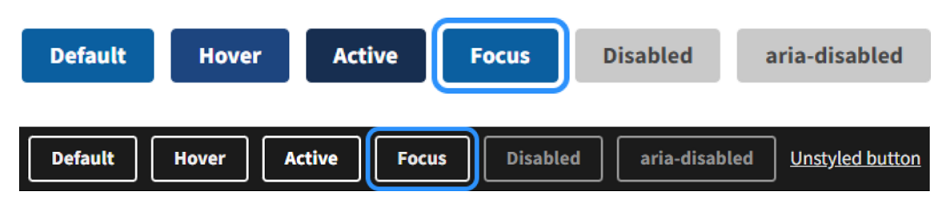
\includegraphics{buttons} \\
Icon List: \href{https://designsystem.digital.gov/components/icon/}{https://designsystem.digital.gov/components/icon/} \\
Alert List: \\
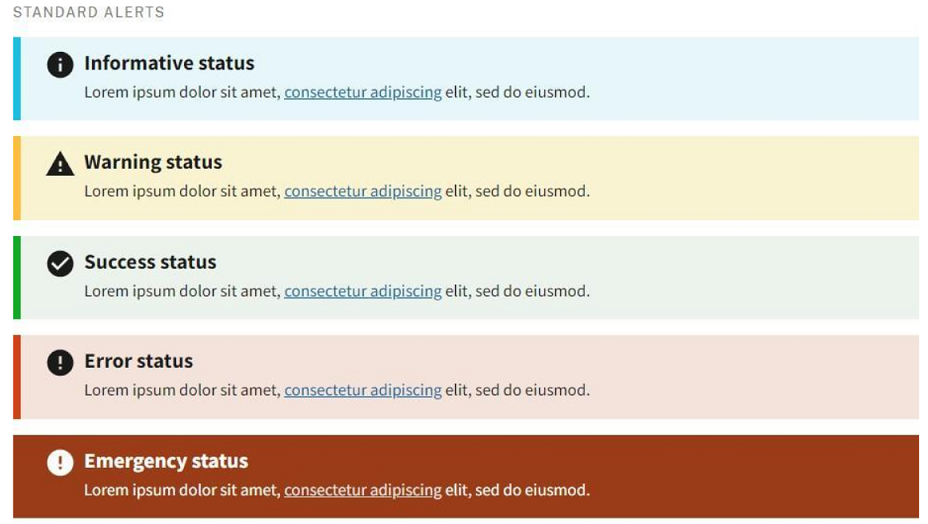
\includegraphics{alerts_1} \\
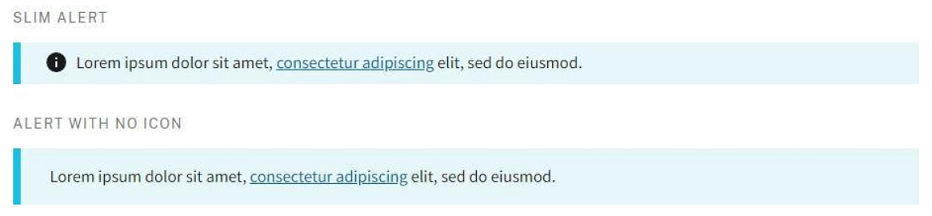
\includegraphics{alerts_2} \\
Headers, Footers, Radio Buttons: \\
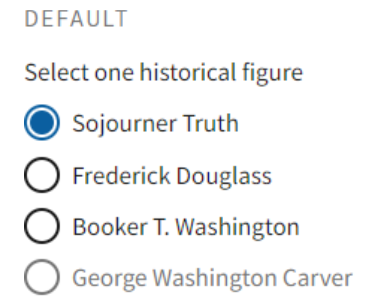
\includegraphics{headers} \\
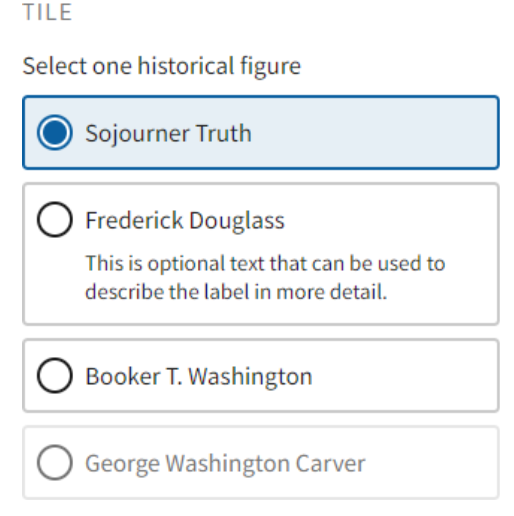
\includegraphics{footers} \\
Select: \\
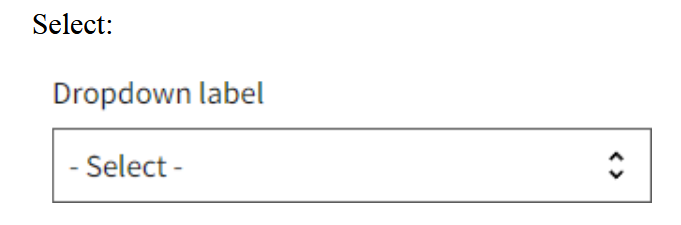
\includegraphics{radiobuttons} \\
Site Alerts: \\
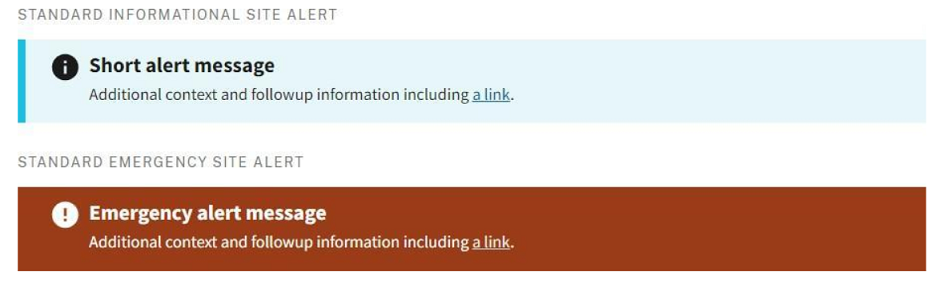
\includegraphics{alerts_site} \\
Step Indicators: \\

\includegraphics{step_indicator} \\
Tags: \\
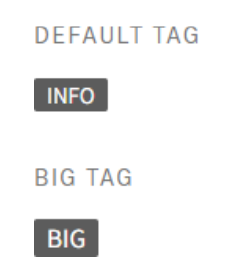
\includegraphics{tags} \\
Text Inputs: \\
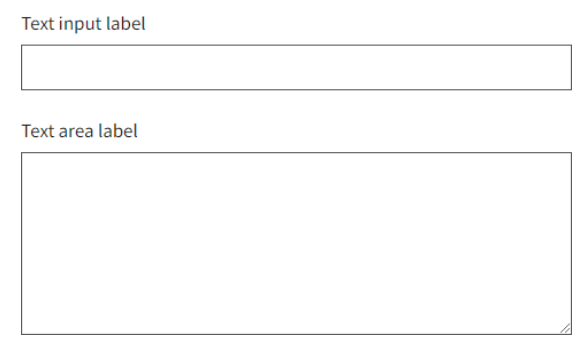
\includegraphics{text_inputs} \\
Typefaces: Source Sans Pro, Public Sans, Roboto Mono, Merriweather

The following images are draft mockups of the landing and scouting pages (not all mockups are finished yet): \\
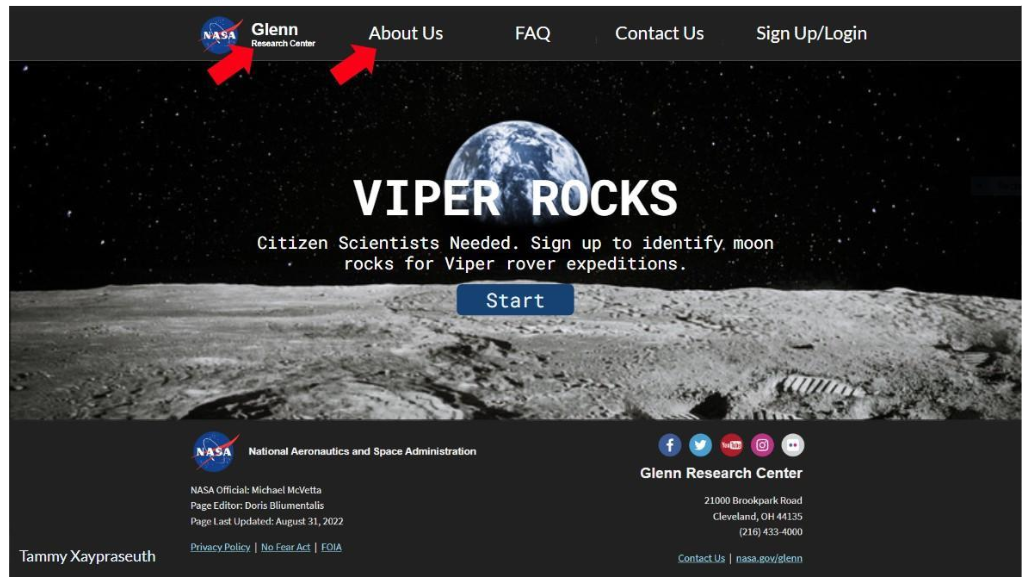
\includegraphics{landing_page_1}
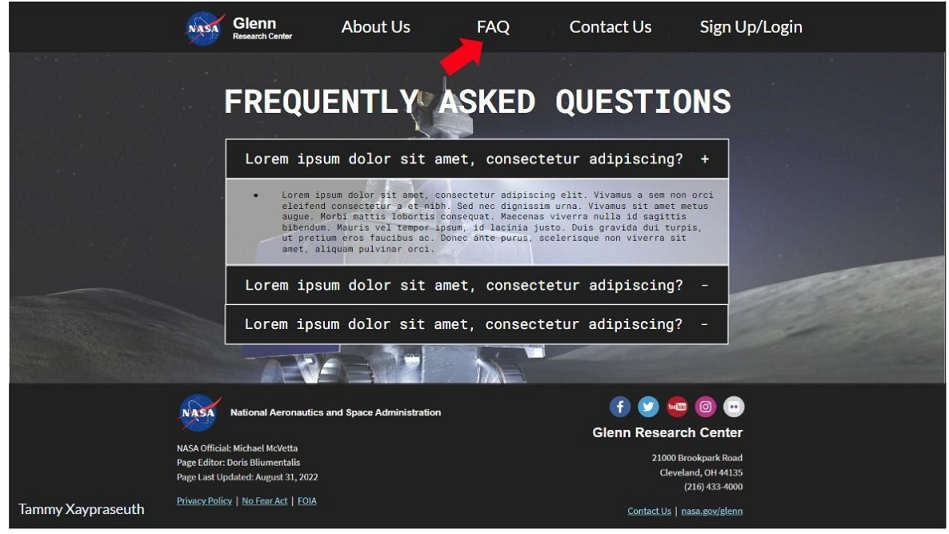
\includegraphics{landing_page_2}
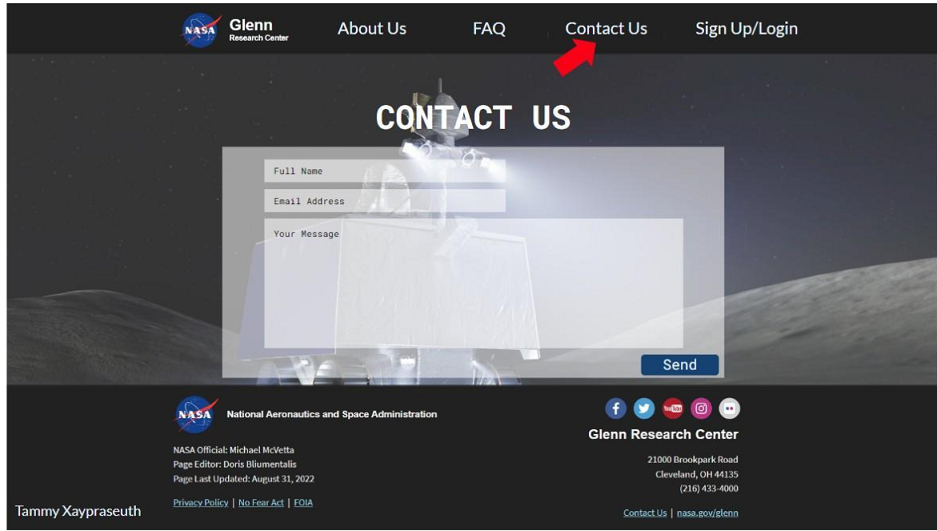
\includegraphics{landing_page_3}
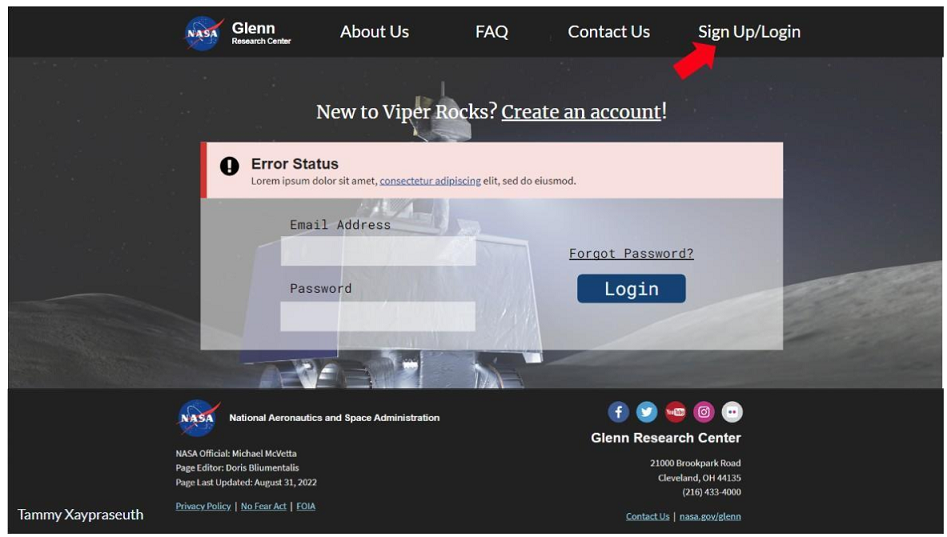
\includegraphics{landing_page_4}
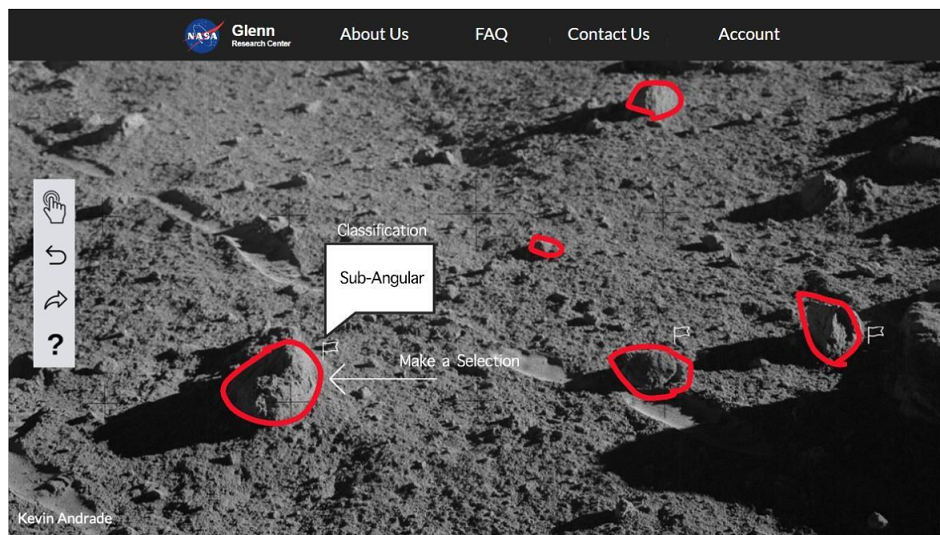
\includegraphics{scouting_page}
As per the Americans with Disabilities Act, we will adhere closely to the following checklist based on the Act’s guidelines:
\begin{enumerate}
	\item Read the law documentation
	\item All media files and maps should have an “alt” tag
	\item All your online forms should have descriptive html tags
	\item All hyperlinks should have a descriptive anchor text
	\item All pages on your website have “skip navigation” links
	\item All the text content should be structured using proper heading tags
	\item All PDF files should be accessible
	\item All videos should have subtitles, transcripts, and audio description
	\item The color contrast of your web pages should be sufficient according to WCAG
	\item All fonts should be accessible
	\item All HTML tables should be populated with column headers, row identifiers, and cell information
	\item All audio files on your website should have a written caption
	\item All call-to-action buttons on your website should have an accessible name and an ARIA label
	\item All your website should be accessible with keyboard navigation
	\item Have a website accessibility policy page
	\item Have easily locatable contact information to allow users to request accessibility information
	\item Test your website accessibility according to the Website Content Accessibility Guidelines
	\item Automate your website accessibility check to prevent missing critical accessibility issues
\end{enumerate}
We will also look to and reference the USWDS and NASA Guidelines for guidance on accessible designs.

\subsection{Hardware Interfaces}
The following are different input systems that will be kept in mind while developing this web application. Users will need a mobile device or personal computer. If they have a personal computer, they will require a mouse and keyboard or a trackpad.
\subsection{Software Interfaces}
The following are software interfaces that will be used for this product
\begin{itemize}
	\item React 18.2.0
	\item MySQL 8.0
	\item MongoDB 7.0
	\item Javascript - version TBD
	\item Node.js 20.17.0 LTS
\end{itemize}
\subsection{Communications Interfaces}
Users will need an email if they choose to contact the team. The team’s emails are listed on the website for anybody to contact.

\section{Legal and Ethical Considerations}
The VIPER Rocks! citizen science project aims to engage the public with lunar science research by collecting and analyzing user-generated data. However, this raises various legal and ethical considerations that must be addressed to ensure the protection of users and the responsible conduct of scientific research.

\textbf{Privacy}:
\begin{itemize}
	\item The project must clearly inform users about the types of data collected through the application and how it will be used.
	\item User consent must be obtained explicitly before collecting any personal information.
	\item Secure data transfer protocols and robust data storage systems must be implemented to prevent unauthorized access.
\end{itemize}

\textbf{Security}: 
\begin{itemize}
	\item The security of the user’s data must be maintained. Methods will be implemented to ensure it stays secure and private.
	\item The project will implement secure user authentication mechanisms to prevent unauthorized access to accounts and data. 
\end{itemize}
The legal and ethical considerations outlined above highlight important issues that must be addressed. It is crucial for us to ensure these concerns are handled properly for the development and operation of the VIPER Rocks! project.

\section{Appendix A: Glossary}
\begin{itemize}
	\item LUNAR - Lunar Uplink for Navigation and Analysis of Reconnaissance
\end{itemize}


\end{document}